\documentclass{article}
\usepackage{natbib,graphicx,dblfloatfix,multirow,array,threeparttable,xspace}
\usepackage[landscape,hmargin=1.5cm,vmargin=1.5cm]{geometry}

\newcommand{\mtwo}{PAML M2a\xspace}
\newcommand{\meight}{PAML M8\xspace}
\newcommand{\pranka}{PRANK$_{\textrm{AA}}$\xspace}
\newcommand{\prankc}{PRANK$_{\textrm{C}}$\xspace}
\newcommand{\omg}{\bm{\omega}\xspace}
\newcommand{\tpr}{TPR$_{1\%}$\xspace}
\newcommand{\tprf}{TPR$_{5\%}$\xspace}
\newcommand{\sw}{sitewise\xspace}
\newcommand{\Sw}{Sitewise\xspace}
\newcommand{\Dr}{{\emph{Drosophila}}\xspace}

\begin{document}

\makeatletter 
\renewcommand{\figurename}{Supplementary Figure}
\renewcommand{\thefigure}{S\@arabic\c@figure} 

\begin{figure}[t]
\begin{center}
%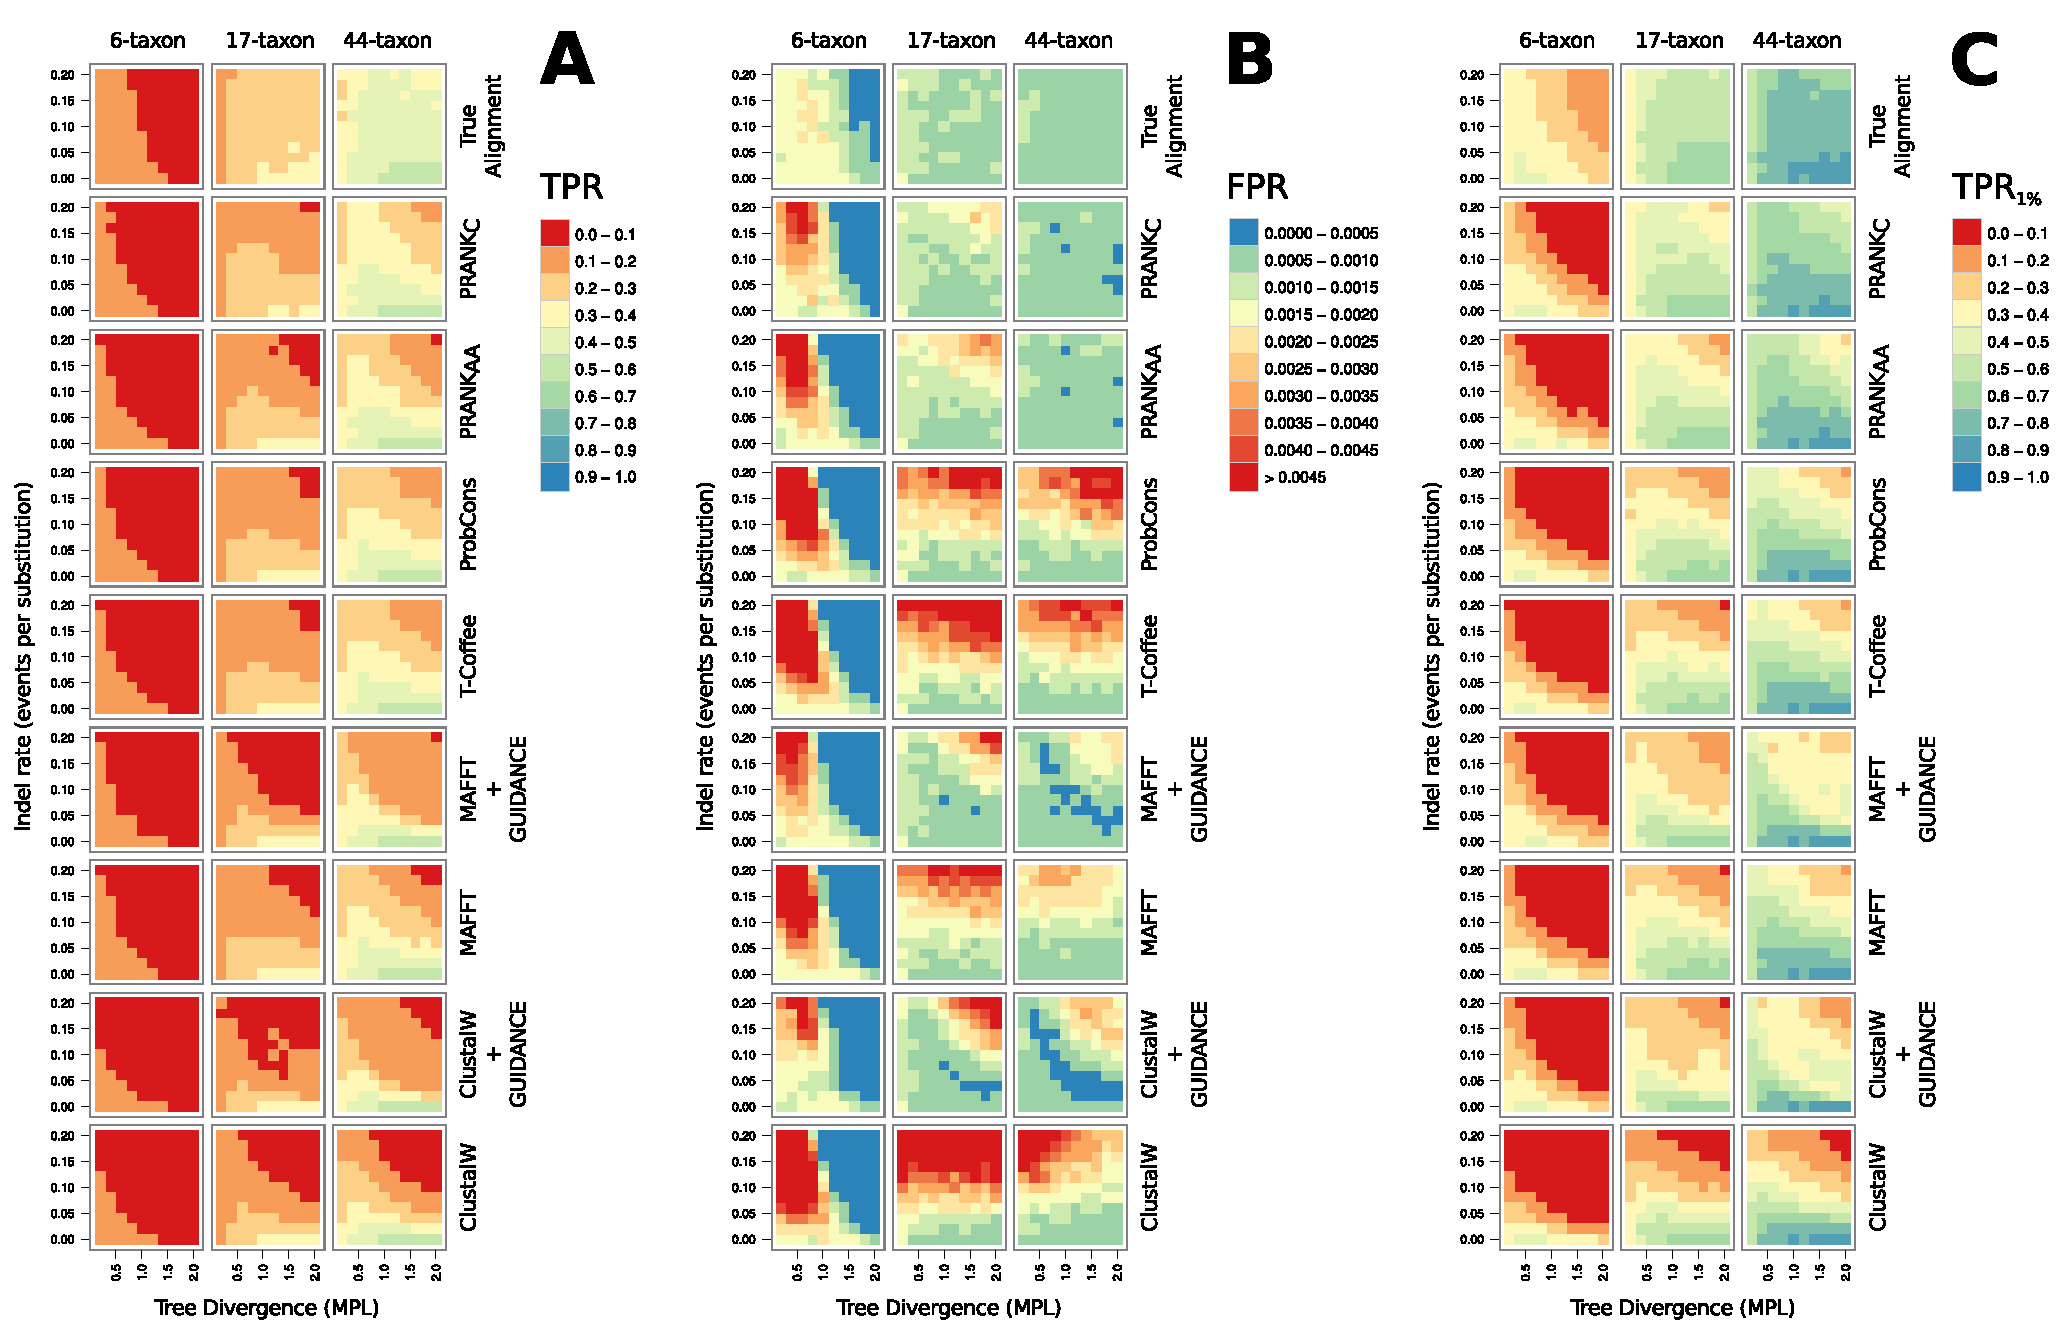
\includegraphics[scale=0.65]{supp_fig1.pdf}
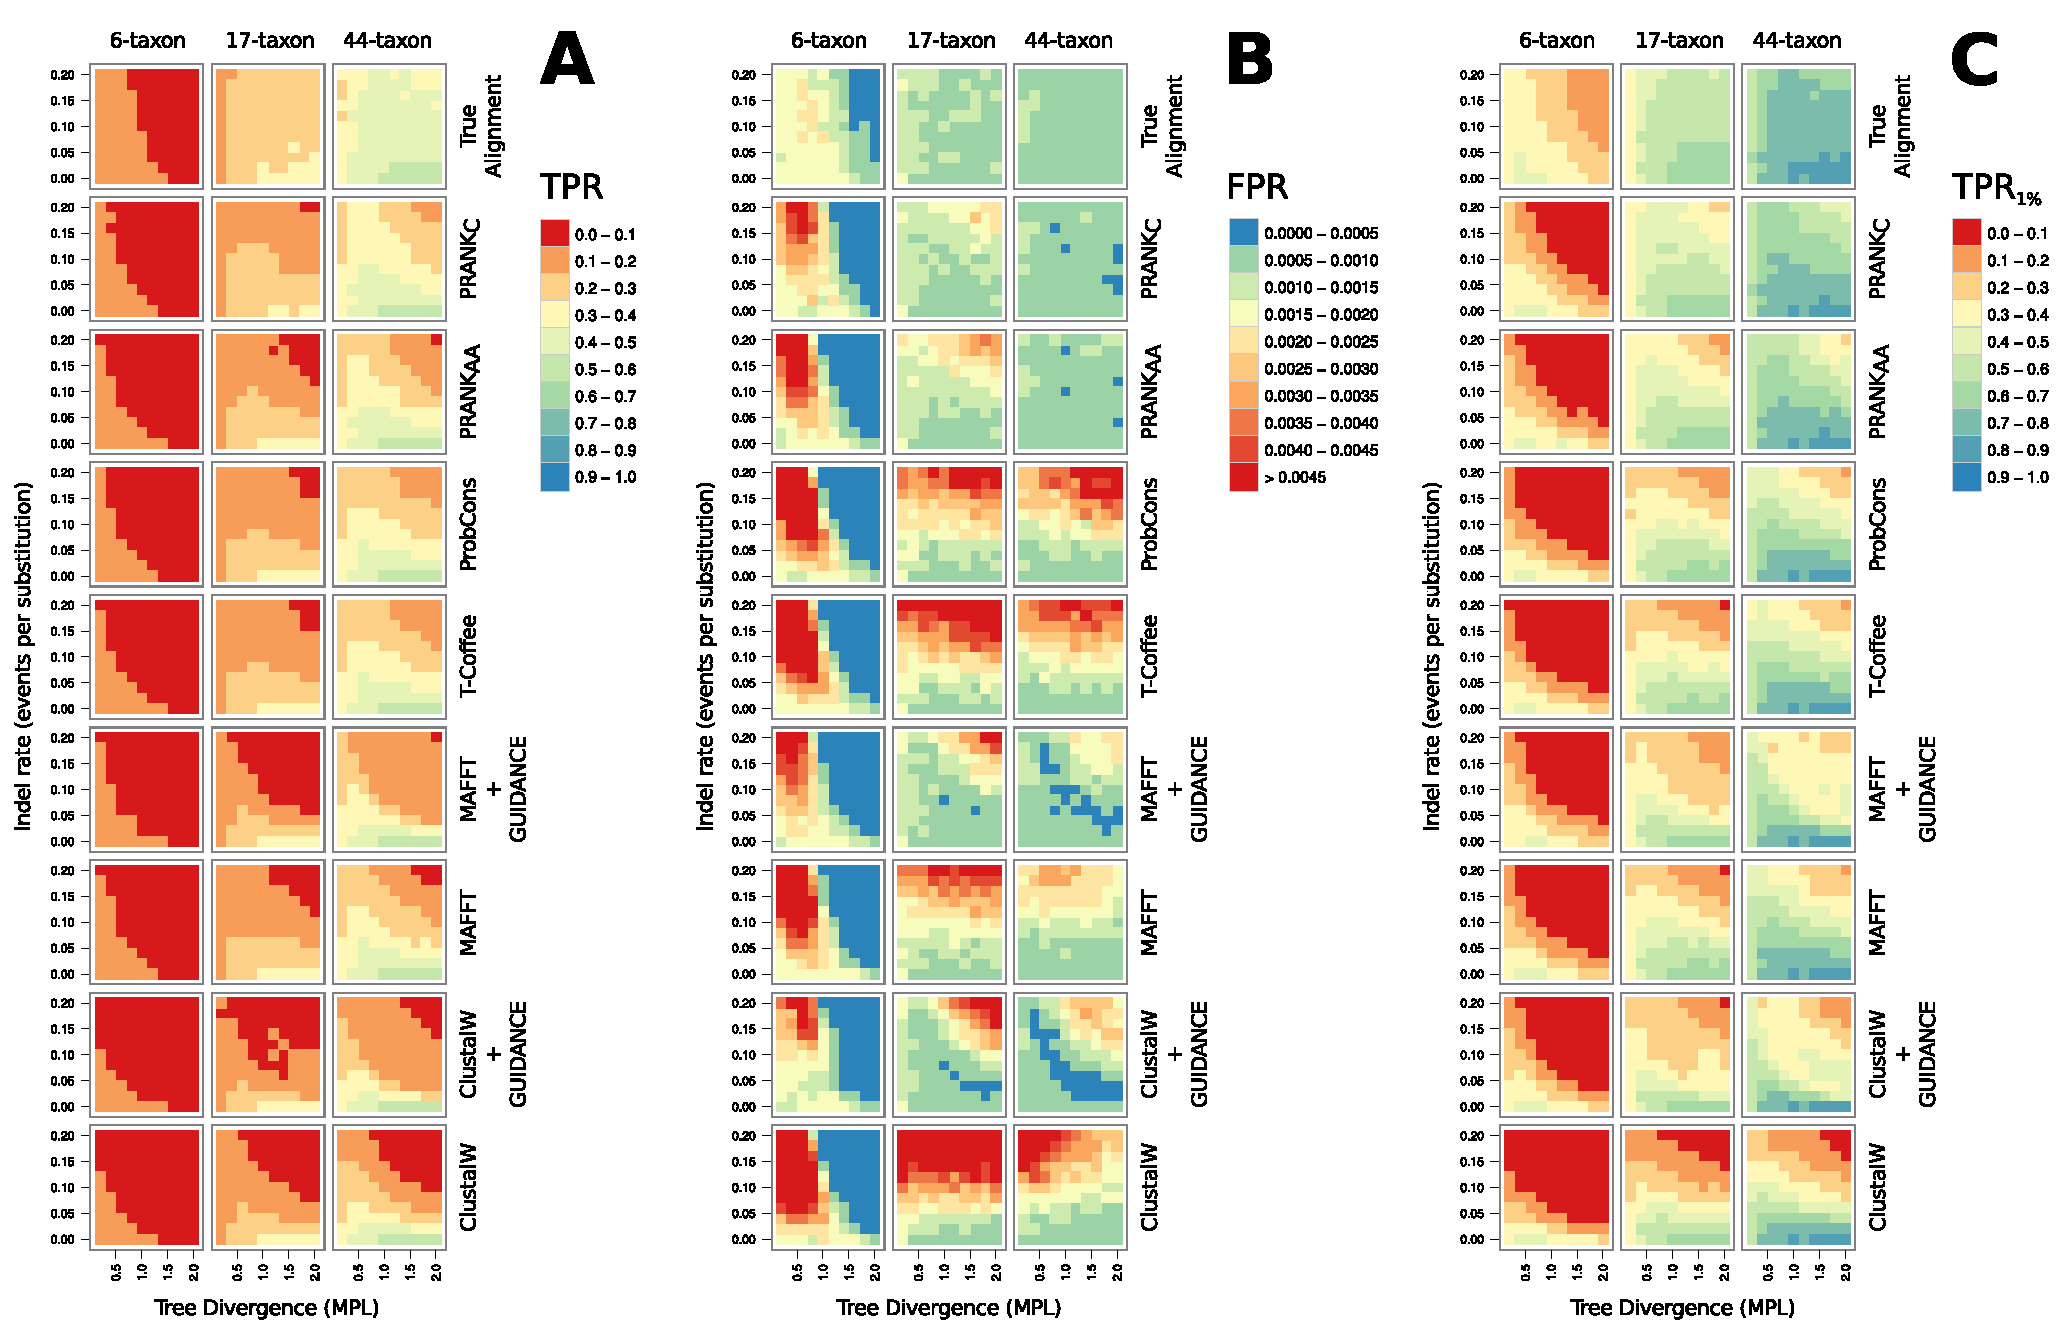
\includegraphics[scale=0.7]{supp_fig1.pdf}
\end{center}
\caption{This figure depicts the same simulations and uses the same
  formatting as Figure 4, except that results for MAFFT and \pranka
  have been added to sections (a) and (b) and results using ClustalW +
  GUIDANCE and MAFFT + GUIDANCE have been added to all sections.}
\label{supp_fig1}
\end{figure}

\begin{figure}[t]
\begin{center}
%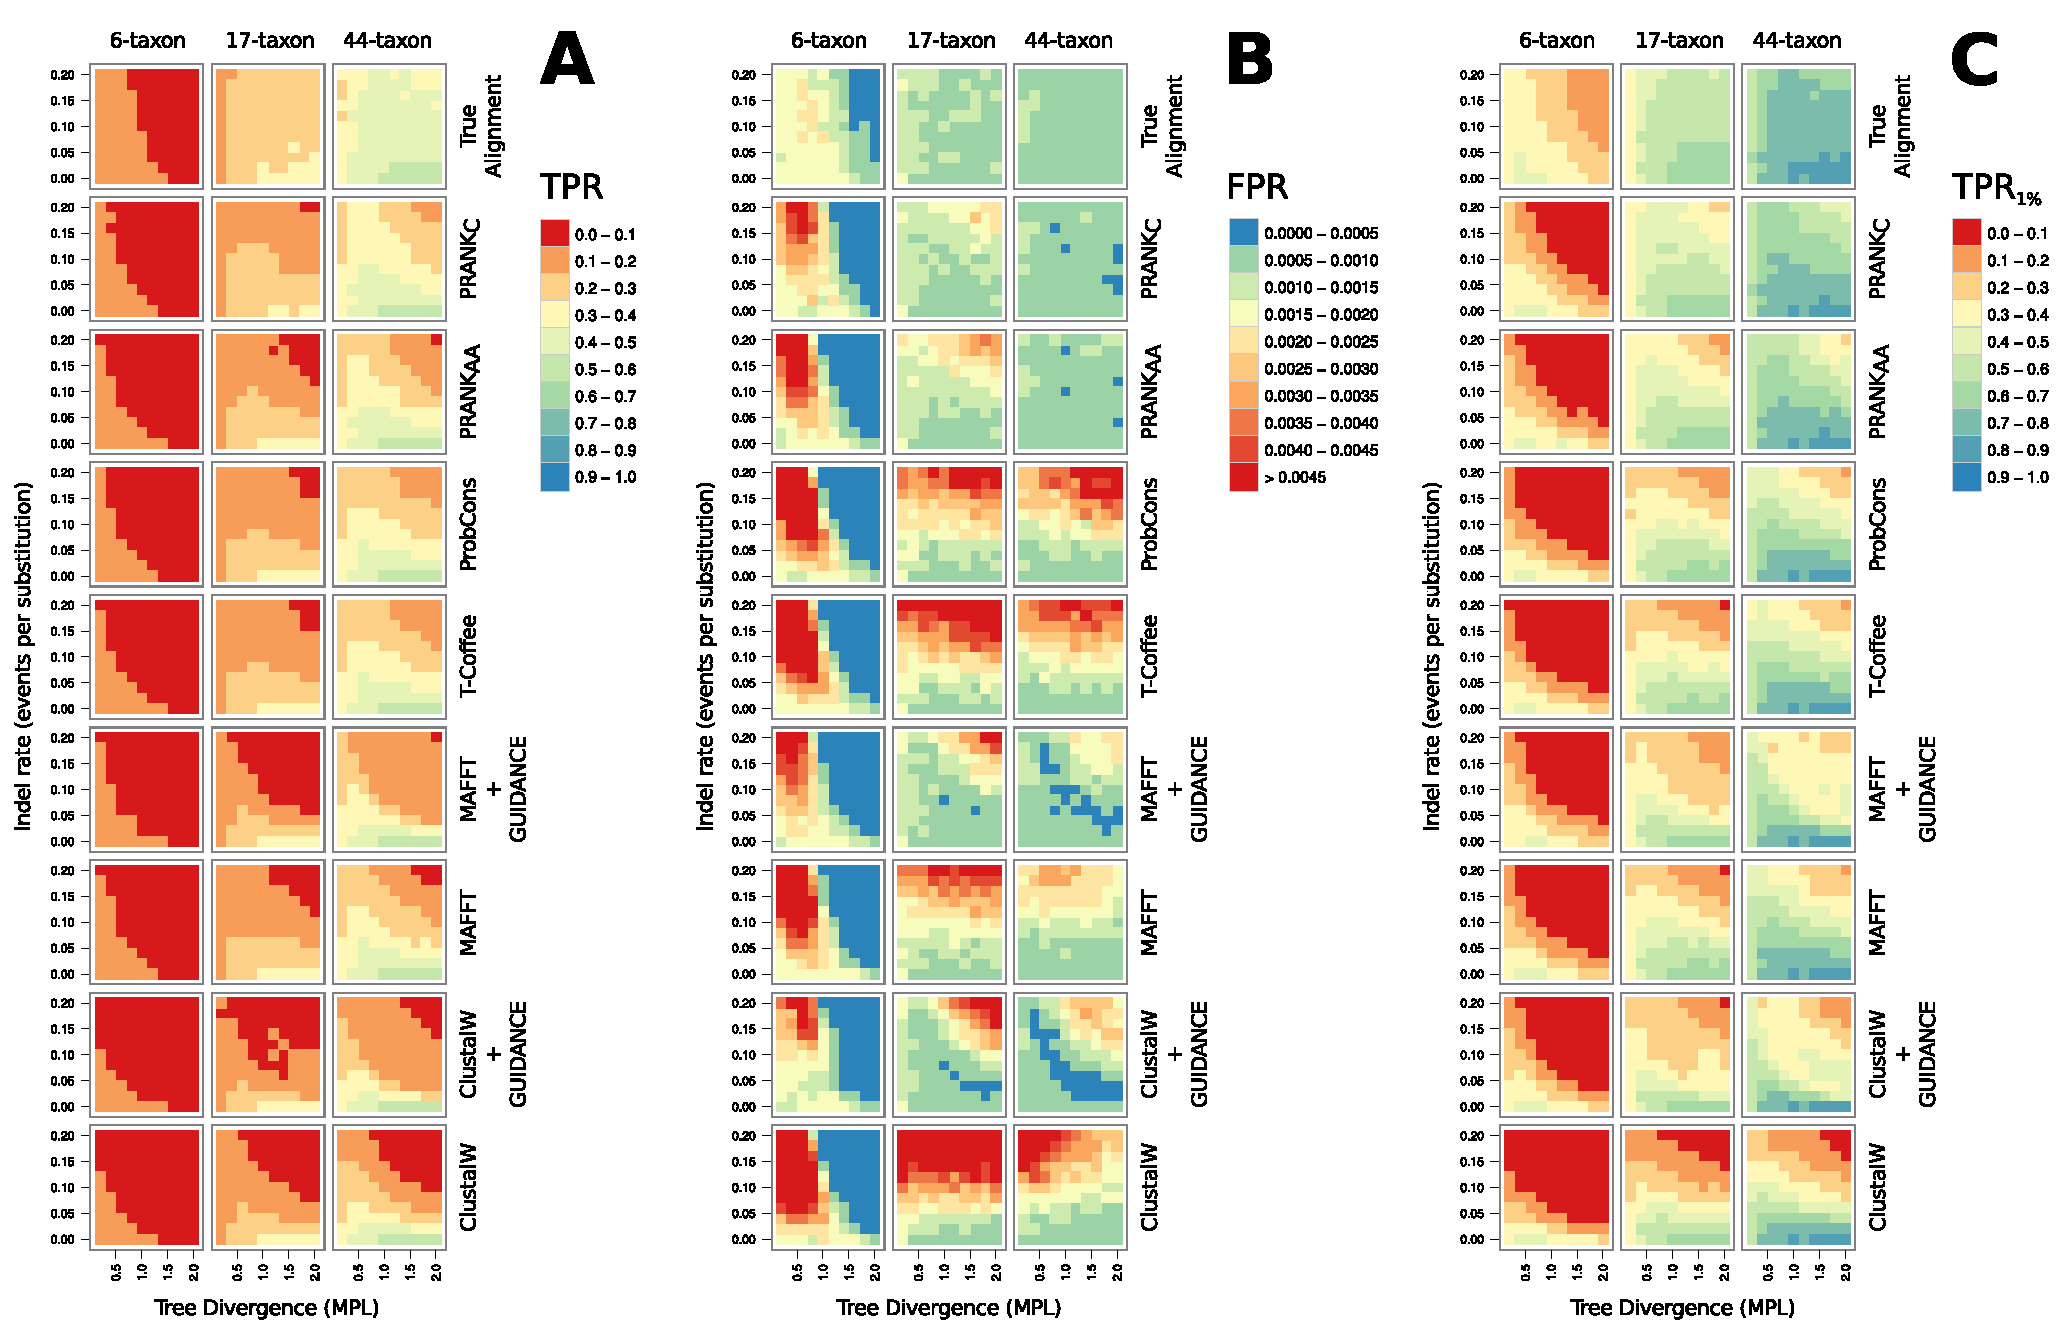
\includegraphics[scale=0.65]{supp_fig1.pdf}
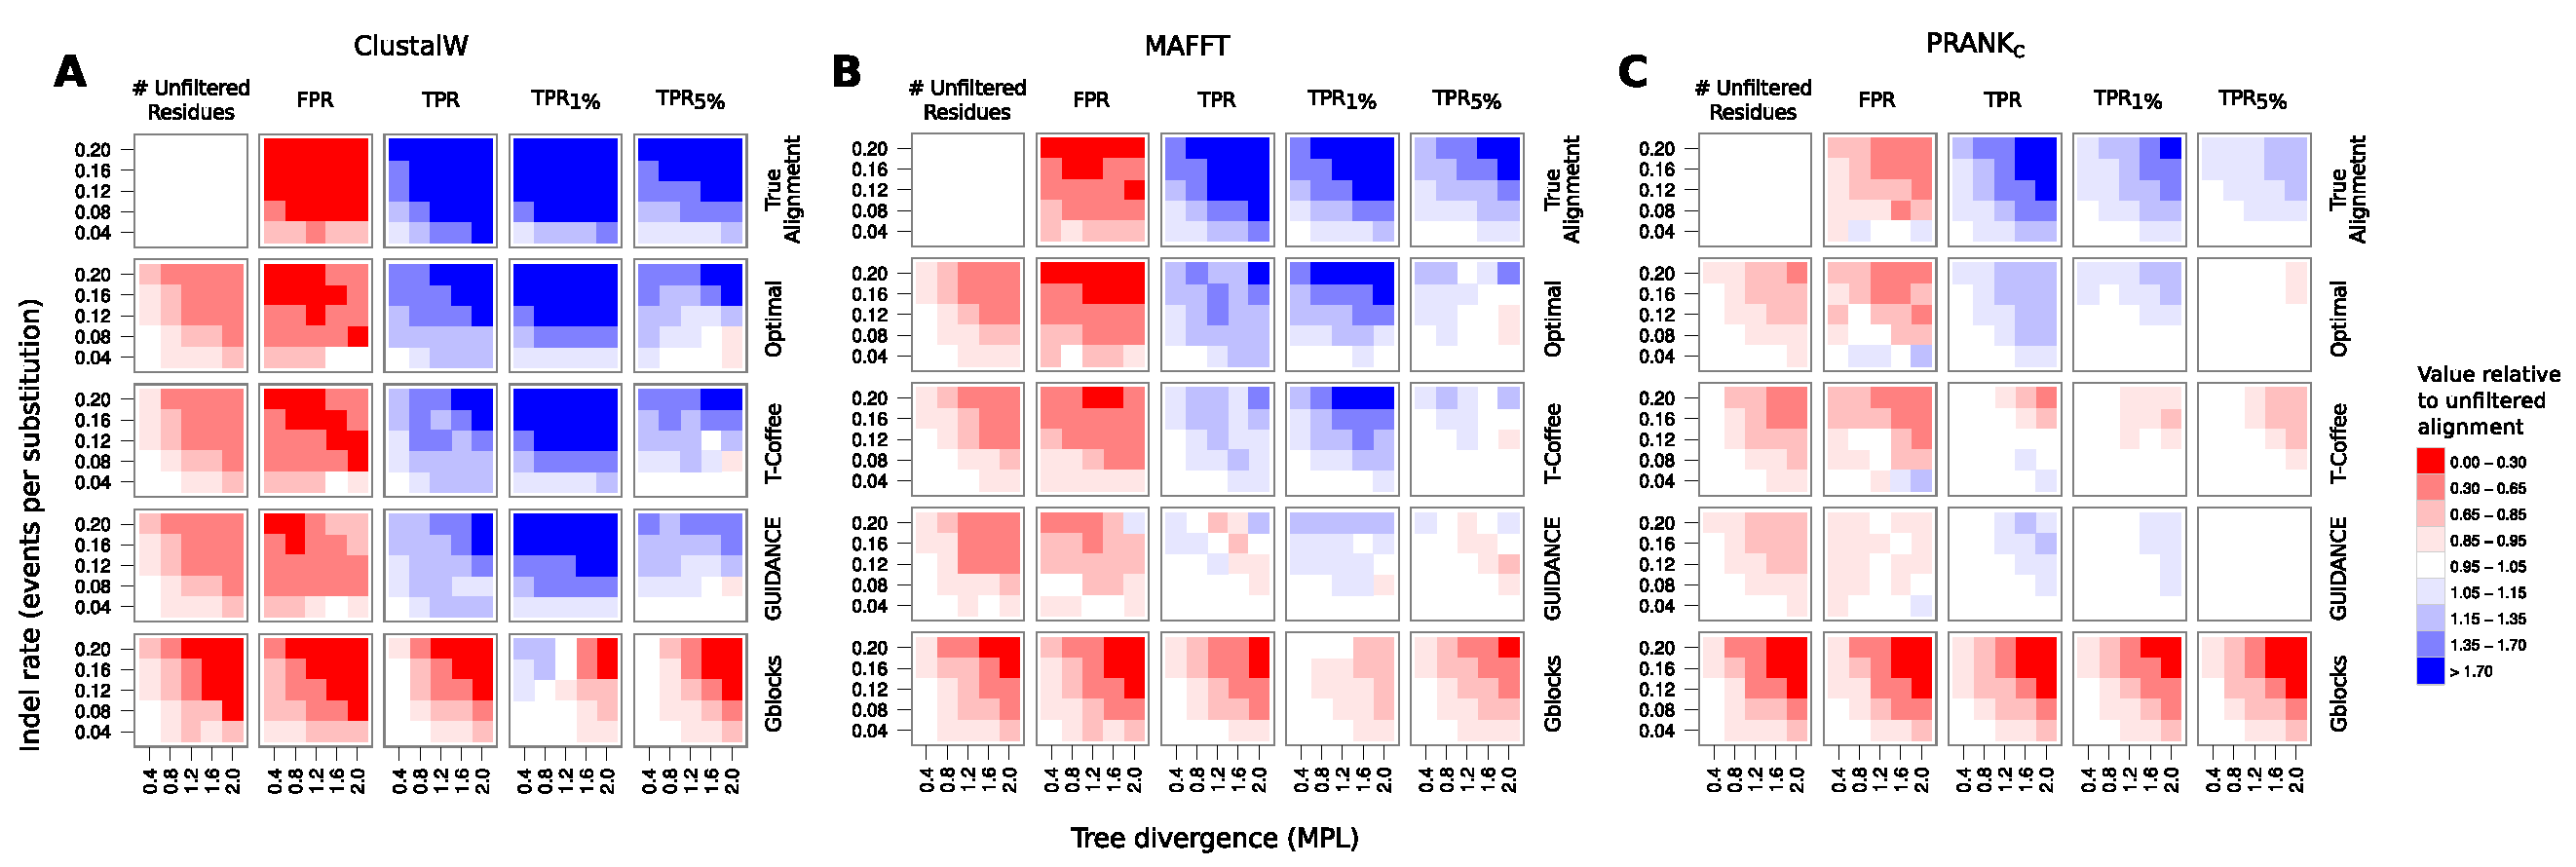
\includegraphics[scale=0.55]{supp_fig2.pdf}
\end{center}
\caption{This figure depicts largely the same simulations and uses the
  same formatting as Figure 5 except for two changes. First,
  results for MAFFT have been added to section (b) and results for
  \prankc have been moved to section (c). Second, the rightmost column
  has been added, showing the true positive rate (TPR) at a 5\% false
  positive rate (FPR) threshold (labeled \tprf).}
\label{supp_fig2}
\end{figure}

\end{document}
